%% The following is a directive for TeXShop to indicate the main file
%%!TEX root = ../diss.tex

\chapter{Applications of oxygen-enhanced MRI}
\label{ch:oemri3}

\section{Preface}

A new term has been introduced in this chapter to compare what has previously been referred to as ``dOE-MRI values''.
The normalized component weighting factor value is now shortened to be \acs{NCWF}.

% ======================================================================
\section{Introduction}
% ======================================================================

Dynamic oxygen-enhanced MRI (\ac{dOE-MRI}) has recently been proposed by our group to assess tumour oxygenation in vivo using MRI~\cite{Moosvi:2018ca}. 
This technique measures T$_1$-weighted changes in tissues in response to a cycling oxygen challenge, with the responsive signals detected using \ac{ICA}. 
Briefly, oxygenation can be assessed \emph{in vivo} by administering a simple gas challenge (switching between two-minute periods of medical air and 100\% O$_2$) during the \ac{dOE-MRI} scan and then using \ac{ICA} to extract the tissue response.
\ac{ICA} is a blind-source separation algorithm that separates multiple signal sources by maximizing statistical independence of individual components~\cite{Hyvarinen:2000vk}.
Various flavours of oxygen-enhanced MRI (OE-MRI) have been proposed but all essentially leverage the paramagnetic properties of inhaled oxygen.
White et al.\ have shown that OE-MRI may be very relevant in developing prognostic factors to predict tumour response to hypofractionation by stratifying tumours that may benefit from oxygen breathing during irradiation~\cite{White:2016fz}.
In this study, we apply \ac{dOE-MRI} to mice bearing tumour xenografts to assess the effect of a common antiangiogenic agent.
We hypothesized that \ac{dOE-MRI} with group-\ac{ICA} can detect \ac{VEGF} ablation-induced changes to oxygenation of SCCVII tumours 48 hours following treatment.

\subsection{VEGF inhibition and bevacizumab}

\acs{VEGF} is a key regulator of angiogenesis as the \acs{VEGF} molecule is rate-limiting in normal and pathological growth of blood vessels.
Bevacizumab is a monocolonal antibody that binds \acs{VEGF} and inhibits growth of blood vessels~\cite{Ferrara:2004fa} and inhibits tumour growth.
It is marketed for clinical use under the name Avastin$^{\tiny{\textrm{\textcopyright}}}$ (Genentech Inc., California, USA) on tumours and its effects and outcomes have been widely reported~\cite{Keating:2014gt, Pavlidis:2013bj, Barnett:2013bt, Kumler:2014gb}.
Tumour xenografts receiving monocolonal antibodies to VEGF have consistently shown reductions in quantitative perfusion parameters from a variety of non-invasive imaging modalities including \acs{DCE-US}~\cite{Wang:2015bb}, \acs{DCE-MRI}~\cite{OConnor:2009cg}, and micro PET~\cite{Nagengast:2007hx}.
For \ac{DCE-US}, Wang et al.\ reported a significant reduction in peak enhancement, area under the curve, relative blood volume, and relative blood flow just 24 hours after a treatment of 10~mg/kg of bevacizumab~\cite{Wang:2015bb}.  
Several \ac{DCE-MRI} animal and human studies have shown reductions in \acs{K$^{trans}$}, \acs{$v_p$}, and \acs{$v_e$} after administration of antiangiogenic agents, including bevacizumab~\cite{Yang:2018hz}.
Tumour growth delay data also clearly indicates that growth is slowed after treatment with bevacizumab~\cite{Yang:2018hz} and other similar \acs{VEGF}-inhibitors~\cite{OConnor:2012ie}.

It is well established that after treatment with antiangiogenic agents, the normalized vasculature is characterized by a reduction in vessel permeability, tortuosity, greater coverage by pericytes and a more normal basement membrane~\cite{Jain:2005gk}. 
These morphological changes often result in functional changes as well including decreased interstitial fluid pressure, increased tumour oxygenation, and improved delivery of nutrients (and drugs)~\cite{Jain:2005gk}.
Bevacizumab is an expensive drug with many adverse effects~\cite{Keating:2014gt} so selective targeting of patients that are most likely to benefit from it should improve its cost-effectiveness~\cite{Barnett:2013bt}.
In this study, we present an exciting application of our non-invasive imaging-based technique with no requirement for an exogenous contrast agent to assess tumour oxygenation before and after treatment with bevacizumab.

% ======================================================================
\section{Methods}
% ======================================================================
\subsection{Animals}
Female NRG (NOD rag gamma) mice were implanted with murine squamous cell carcinoma (SCCVII; $5\times 10^5$ cells in 50~$\mu$l serum-free media; cells provided by Dr.\ J.\ Evans) in the dorsal subcutaneous region.
Tumours were imaged when their largest diameters reached approximately 8-10~mm.
All mice were injected with 60~mg/kg pimonidazole hydrochloride (HypoxyProbe) 30~min prior to imaging to label hypoxic cells and were euthanized within 15~min of imaging completion.
Mice were anesthetized with isoflurane using 1.5-2.0\% isoflurane for the duration of MR imaging sessions until euthanasia, and were positioned supine on the custom surface coil apparatus.
Throughout the imaging session, a small animal monitoring system (SA Instruments Inc., Stony Brook, NY, USA) was used to monitor respiration rate, varying between 80-100~breaths per minute, and body temperature, maintained at ${36.8\pm 0.5^\circ}$C using a continuous airflow heater. 
Tumours were embedded and frozen in optimum cutting temperature medium (OCT; Tissue-TEK).


\subsection{Immunohistochemistry}
As previously described in Section~\ref{doemri_histo}.

\subsection{MR Imaging}
As previously described in Section~\ref{doemri_mrianalysis1}.
All scans were acquired with the same spatial resolution and geometry and an experienced operator outlined the tumour on each slice of the RARE image to construct the region of interest (\acs{ROI}) for each animal and then transferred to all other scans.
Tumour volumes were measured by multiplying individual voxel volume ($0.3\times 0.3\times 0.1$~mm$^3$) and the count of total number of voxels included within the manually drawn \acs{ROI}.

% Imaging was performed using a 7T scanner (Bruker Biospec) with a transmit quadrature volume coil and a custom built surface receive coil. 
% An axial RARE image was acquired to localize the tumour (T$_E$/T$_R$=10.7/4250, RARE factor 8) and a T$_1$ map was acquired using the Look-Locker method. We acquired
% \acs{dOE-MRI} scans using a 2D multi-slice FLASH-based sequence for a total scan time of about 14~min.
% During the \ac{dOE-MRI} scan, breathing gas was alternated between medical air and 100\% oxygen every 2 minutes using a 3-channel gas mixer (CWE, Philadelphia, USA) for a total of 3 air-oxygen-air cycles.

\subsection{\ac{dOE-MRI} Analysis}

As previously described in Section~\ref{doemri_mrianalysis2}.
%%%%
% A suite of in-house software was developed using the python machine learning library scikit-learn~\cite{Pedregosa:2011tv}, specifically \texttt{sklearn.decomposition.FastICA} based on the technique described by Hyvarinen~\cite{Hyvarinen:2000vk}.
% The Fast\ac{ICA} algorithm is applied to serially acquired T$_1$W images and the output is a paired set of components and weighting factors for each voxel in the dataset.
% The deflation-based Fast\ac{ICA} (python package scikit.sklearn v0.17.1) was used to analyze the data. 
% Extracted independent components are not ordered and while the component selection can be automated, in this study an observer was assigned to select the appropriate component.
% The number of independent components for each imaging session was chosen by the operator and ranged from 4-9 to ensure the cyclic behaviour of the T$_1$W signal intensity corresponding to the gas challenge appeared in only one component. 
% The \ac{dOE-MRI} maps were obtained by dividing the \ac{ICA} weighting-factor maps by the mean signal-intensity maps to obtain a spatial map for the strength of a particular voxel's contribution to the component of interest.
Briefly, in these \ac{dOE-MRI} maps, voxels are coloured to indicate the amount by which a given pixel intensity time course is modulated by the oxygen-related component.
To compare \ac{dOE-MRI} maps between mice with different temporal resolutions, a scaling factor was applied as discussed previously (see section~\ref{sec:correctionfactor}).
Final normalized \ac{dOE-MRI} maps were obtained by dividing each pixel of the component map for each animal with the mean signal-intensity over time of the corresponding pixel in the \ac{dOE-MRI} scan. 
Mean normalized component weighting factor (\acs{NCWF}) are reported as a marker for tumour oxygenation with high values indicating increased oxygenation while negative values suggest decreased oxygenation or increased levels of hypoxia. 
Mann-Whitney U non-parametric tests are used to assess the difference between experimental groups and Hedge's $g$ was calculated to determine effect size when $p<0.05$.
%The green-white-purple colour spectrum depicts the degree to which voxels respond to the cycled gas challenge.
%Purple indicates O$_2$-positive voxels whose time course exhibits a higher and more positive contribution from the corresponding \ac{ICA} component, representing an increase in T$_1$W signal intensity in response to the supplied 100\% oxygen, and corresponding to areas with excess dissolved oxygen.
%O$_2$-negative voxels that show a decrease in T$_1$W signal intensity with a negative contribution from the corresponding \ac{ICA} component under 100\% oxygen breathing are depicted as green. 
%Regions whose T$_1$W signal intensity time courses responds only weakly or not at all to the gas challenge are shown in white hues.
%A feature of Fast\ac{ICA} is that the norm of each component is normalized to 1 ($||c_i||=1, \forall i$) and the corresponding weighting factor map carries the scaling factor.

\subsection{Experiment Summaries}
General methods common to both experiments have been described above, below are implementation details for each of the two separate experiments presented in this study.

\subsubsection{Experiment 1: Evaluating the utility of dOE-MRI to assess oxygenation improvements after anti-VEGF ablation therapy}
\label{sec:B20_expt1}
\noindent\textbf{Animals}: Seventeen (17) mice were implanted for this experiment with eight left untreated and nine mice treated with 5mg/kg mouse anti-VEGF antibody (B20-4.1.1, Genentech) 48 hours prior to imaging.

\noindent\textbf{MRI}: Axial \ac{dOE-MRI} scans were acquired with 90 repetitions using a 2D FLASH based sequence with T$_E$/T$_R$=2.67/133 ms, flip angle $\alpha$=40$^\circ$, 16 slices each 1mm thick, FOV of 3.84cm x 2.16 cm, encoding matrix of 128x72, and a temporal resolution of 9.6s for a total scan time of about 14 minutes.

\subsubsection{Experiment 2: Assessing oxygenation changes in intramuscular and subcutaneous tumours Anti-VEGF ablation therapy in \acs{IM} vs. \acs{SC} tumours}
\noindent\textbf{Animals}: Thirteen (13) mice were used in this experiment. 
3 mice were implanted with SCCVII in the dorsal subcutaneous (SC) region.
10 mice were implanted in both the dorsal subcutaneous (SC) as well as in the hind limb intramuscular (IM) region.
To account for the accelerated rate of growth for tumours implanted intramuscularly, one-fifth of the cells were implanted \acs{IM} (1x10$^5$ cells in 50$\mu$l serum-free media).
Separate ROIs were drawn on the T$_2$W images to outline both the \acs{SC} and \acs{IM} tumours.
5 mice were treated with 5mg/kg B20 24 hours prior to imaging and 8 were untreated controls.

\noindent\textbf{MRI}: Coronal images were acquired to enable simultaneous imaging of both tumours in the same field of view.
All \ac{dOE-MRI} scans were acquired using a 2D FLASH based sequence with TE = 2.67~ms, spatial resolution $0.3\times 0.3\times 1$~mm$^3$ and flip angle $\alpha=40^\circ$.
To accommodate additional slices and image both tumours in the same scan while maintaining spatial resolution, not all imaging parameters in the \ac{dOE-MRI} scan could be fixed. 
Table~\ref{scanparams} summarizes the key differences in the acquisition parameters for all \ac{dOE-MRI} sequences used in experiment 2.

\begin{table}[htbp]
\centering
\begin{tabular}{c|c|c|c|c|c}
Experiment & Mice & TR/ms & Slices & Repetitions & Temporal resolution (ms)\\
\hline
 1 & 17& 133 & 16 & 90  & 9.6  \\
 2 & 5 & 133 & 16 & 110 & 8.5  \\
 2 & 8 & 83  & 10 & 140 & 6.7 \\
\end{tabular}
\caption{Summary of scan parameters for the experiments used in this study.}
\label{scanparams}
\end{table}

% ======================================================================
\section{Results} 
% ======================================================================

\subsection{Subcutaneously implanted SCCVII tumours treated with B20 are more responsive to oxygen than controls}

Visual inspection of \ac{dOE-MRI} parameter maps in Figure~\ref{dOEMRImaps} show that treatment of SCCVII tumours with the anti-angiogenic agent B20 resulted in an increased oxygenation compared to untreated controls.
Tumours in this experiment were treated 48 hours prior to imaging.
Group differences are shown in Figure~\ref{aarts3boxplot} as a standard box plot; Eight control tumours had a mean \acs{NCWF} value of 0.037$\pm$0.011 and nine treated tumours had a mean of 0.094$\pm$0.037.
This difference was statistically significantly different (Mann-Whitney $U = 11 , p = 0.0092$) and the effect size was large with Hedge's ${g=1.08}$.
Considerable heterogeneity was observed between mice and within a single slice (Fig.~\ref{dOEMRImaps}).
A histogram of voxels within tumour \acs{ROI}s for all mice is shown in Fig.~\ref{aarts3boxplot}B.

\begin{figure}[htbp]
   \centering
   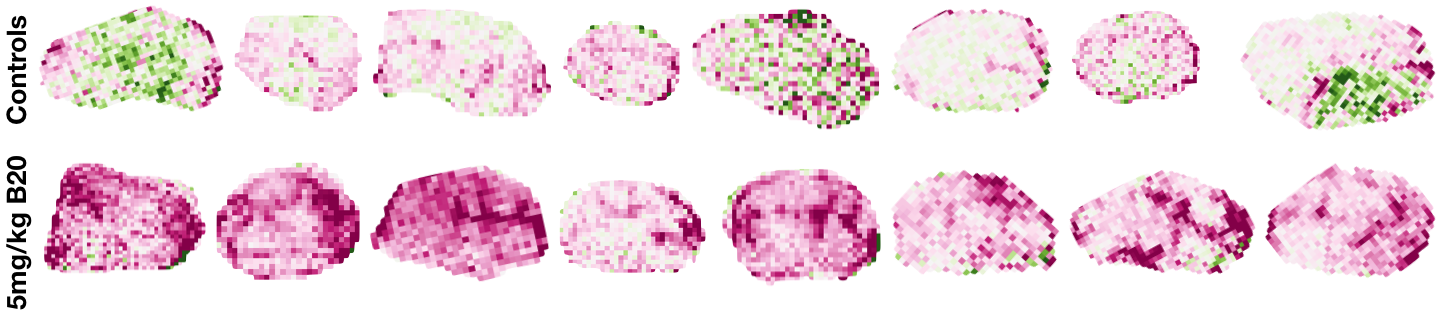
\includegraphics[width=\textwidth]{oemri_thesis3/oemri_thesis3-images/1_aarts3_b20_dOEMRI.pdf} % requires the graphicx package
   \caption{A) \acs{NCWF} maps obtained from \ac{ICA} (\ac{dOE-MRI} maps) are shown for control tumours as well as those treated with 5mg/kg B20 and imaged 48 hours later.
   Of the 10-16 slices for each animal, a representative slice was chosen.
   As indicated by the distribution of purple voxels, control tumours show considerably less response to oxygen than the treated tumours.
   Additionally, regions marked in green are considered to be hypoxic; these regions were not prevalent in the treated tumours.
   B) A representative histology slice from a control and a treated tumour is shown stained with pimonidazole (green) and CD31 (purple).}
   \label{dOEMRImaps}
\end{figure}

\begin{figure}[htbp]
   \centering
   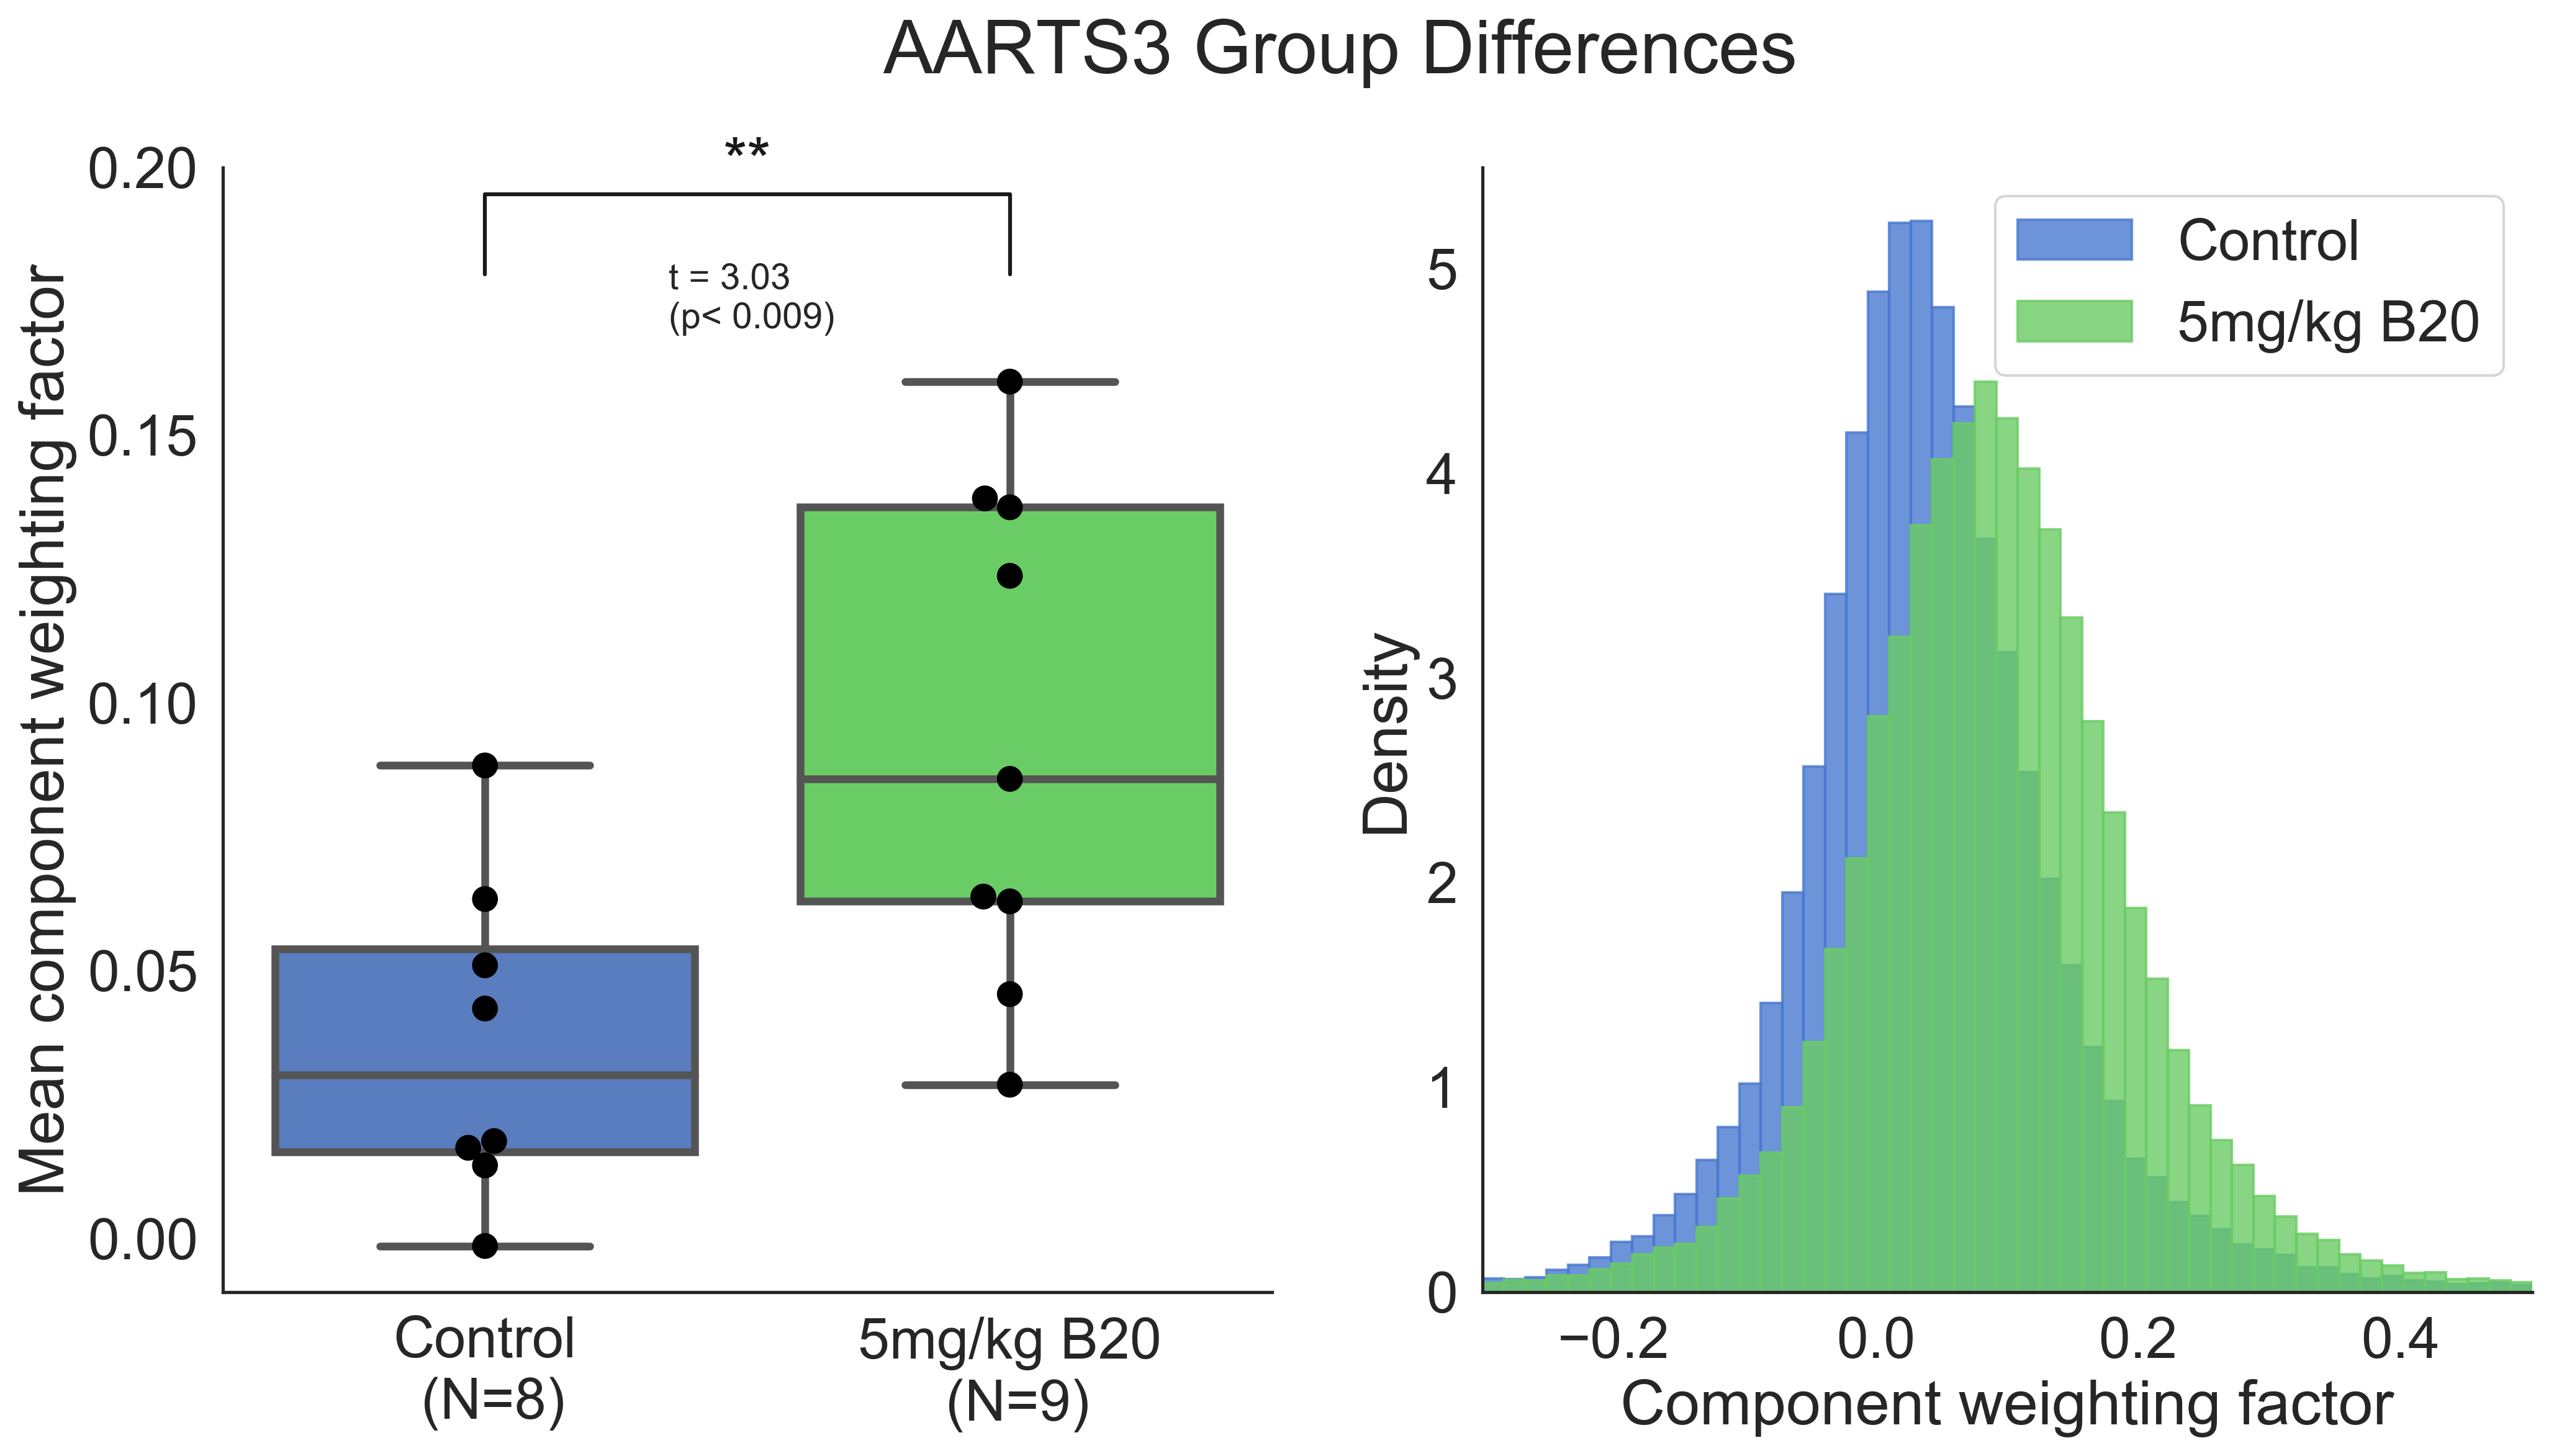
\includegraphics[width=\textwidth]{oemri_thesis3/oemri_thesis3-images/2_aarts3_b20_boxplot_dOEMRI.png} % requires the graphicx package
   \caption{A) Group differences of the normalized mean \acs{NCWF} are shown in a boxplot.
   Each dot represents the mean value of a mouse with the controls in blue and treated in green.
   The differences are statistically significantly different (p=0.0092) with a large effect size (Hedge's g = 1.08).
   B) Density distributions of all voxels shows treated tumours shifting towards increased responsiveness to delivered oxygen (higher \acs{NCWF}).}
   \label{aarts3boxplot}
\end{figure}

\subsection{\acs{IM} tumours have a higher baseline oxygenation level than \acs{SC} tumours from the same cell line}

Tumours implanted at the \acs{IM} site received only 20\% of the cells compared to the subcutaneous tumours to account for faster growth of \acs{IM} tumours.
Figure~\ref{tumourVolumes} shows no statistically significant difference in tumour volumes for any of the groups, control or treated, \acs{IM} or \acs{SC}. 
Across 10 animals and 23 tumours in total, the mean across all groups was $V = 424 \pm 41 mm^3$ (mean $\pm$ sem). 
%Histological sections of the \acs{IM} and \acs{SC} tumours show the microenvironments to be morphologically distinct (figure~\ref{imsc}).\todo[backgroundcolor=red!20!white]{add a couple of sentences about differences in morphology}.
\ac{dOE-MRI} was applied to mice bearing both \acs{SC} and \acs{IM} tumours to evaluate whether tumour implant site affects baseline oxygenation. 
As shown in figure~\ref{OEP8boxplot}, baseline \acs{NCWF} values in \acs{IM} tumours were significantly higher for \acs{IM} tumours compared to \acs{SC} tumours (Mann-Whitney U = 1.0, p = 0.003).
The effect size was large with Hedge's ${g=1.38}$.

\begin{figure}[htbp]
   \centering
   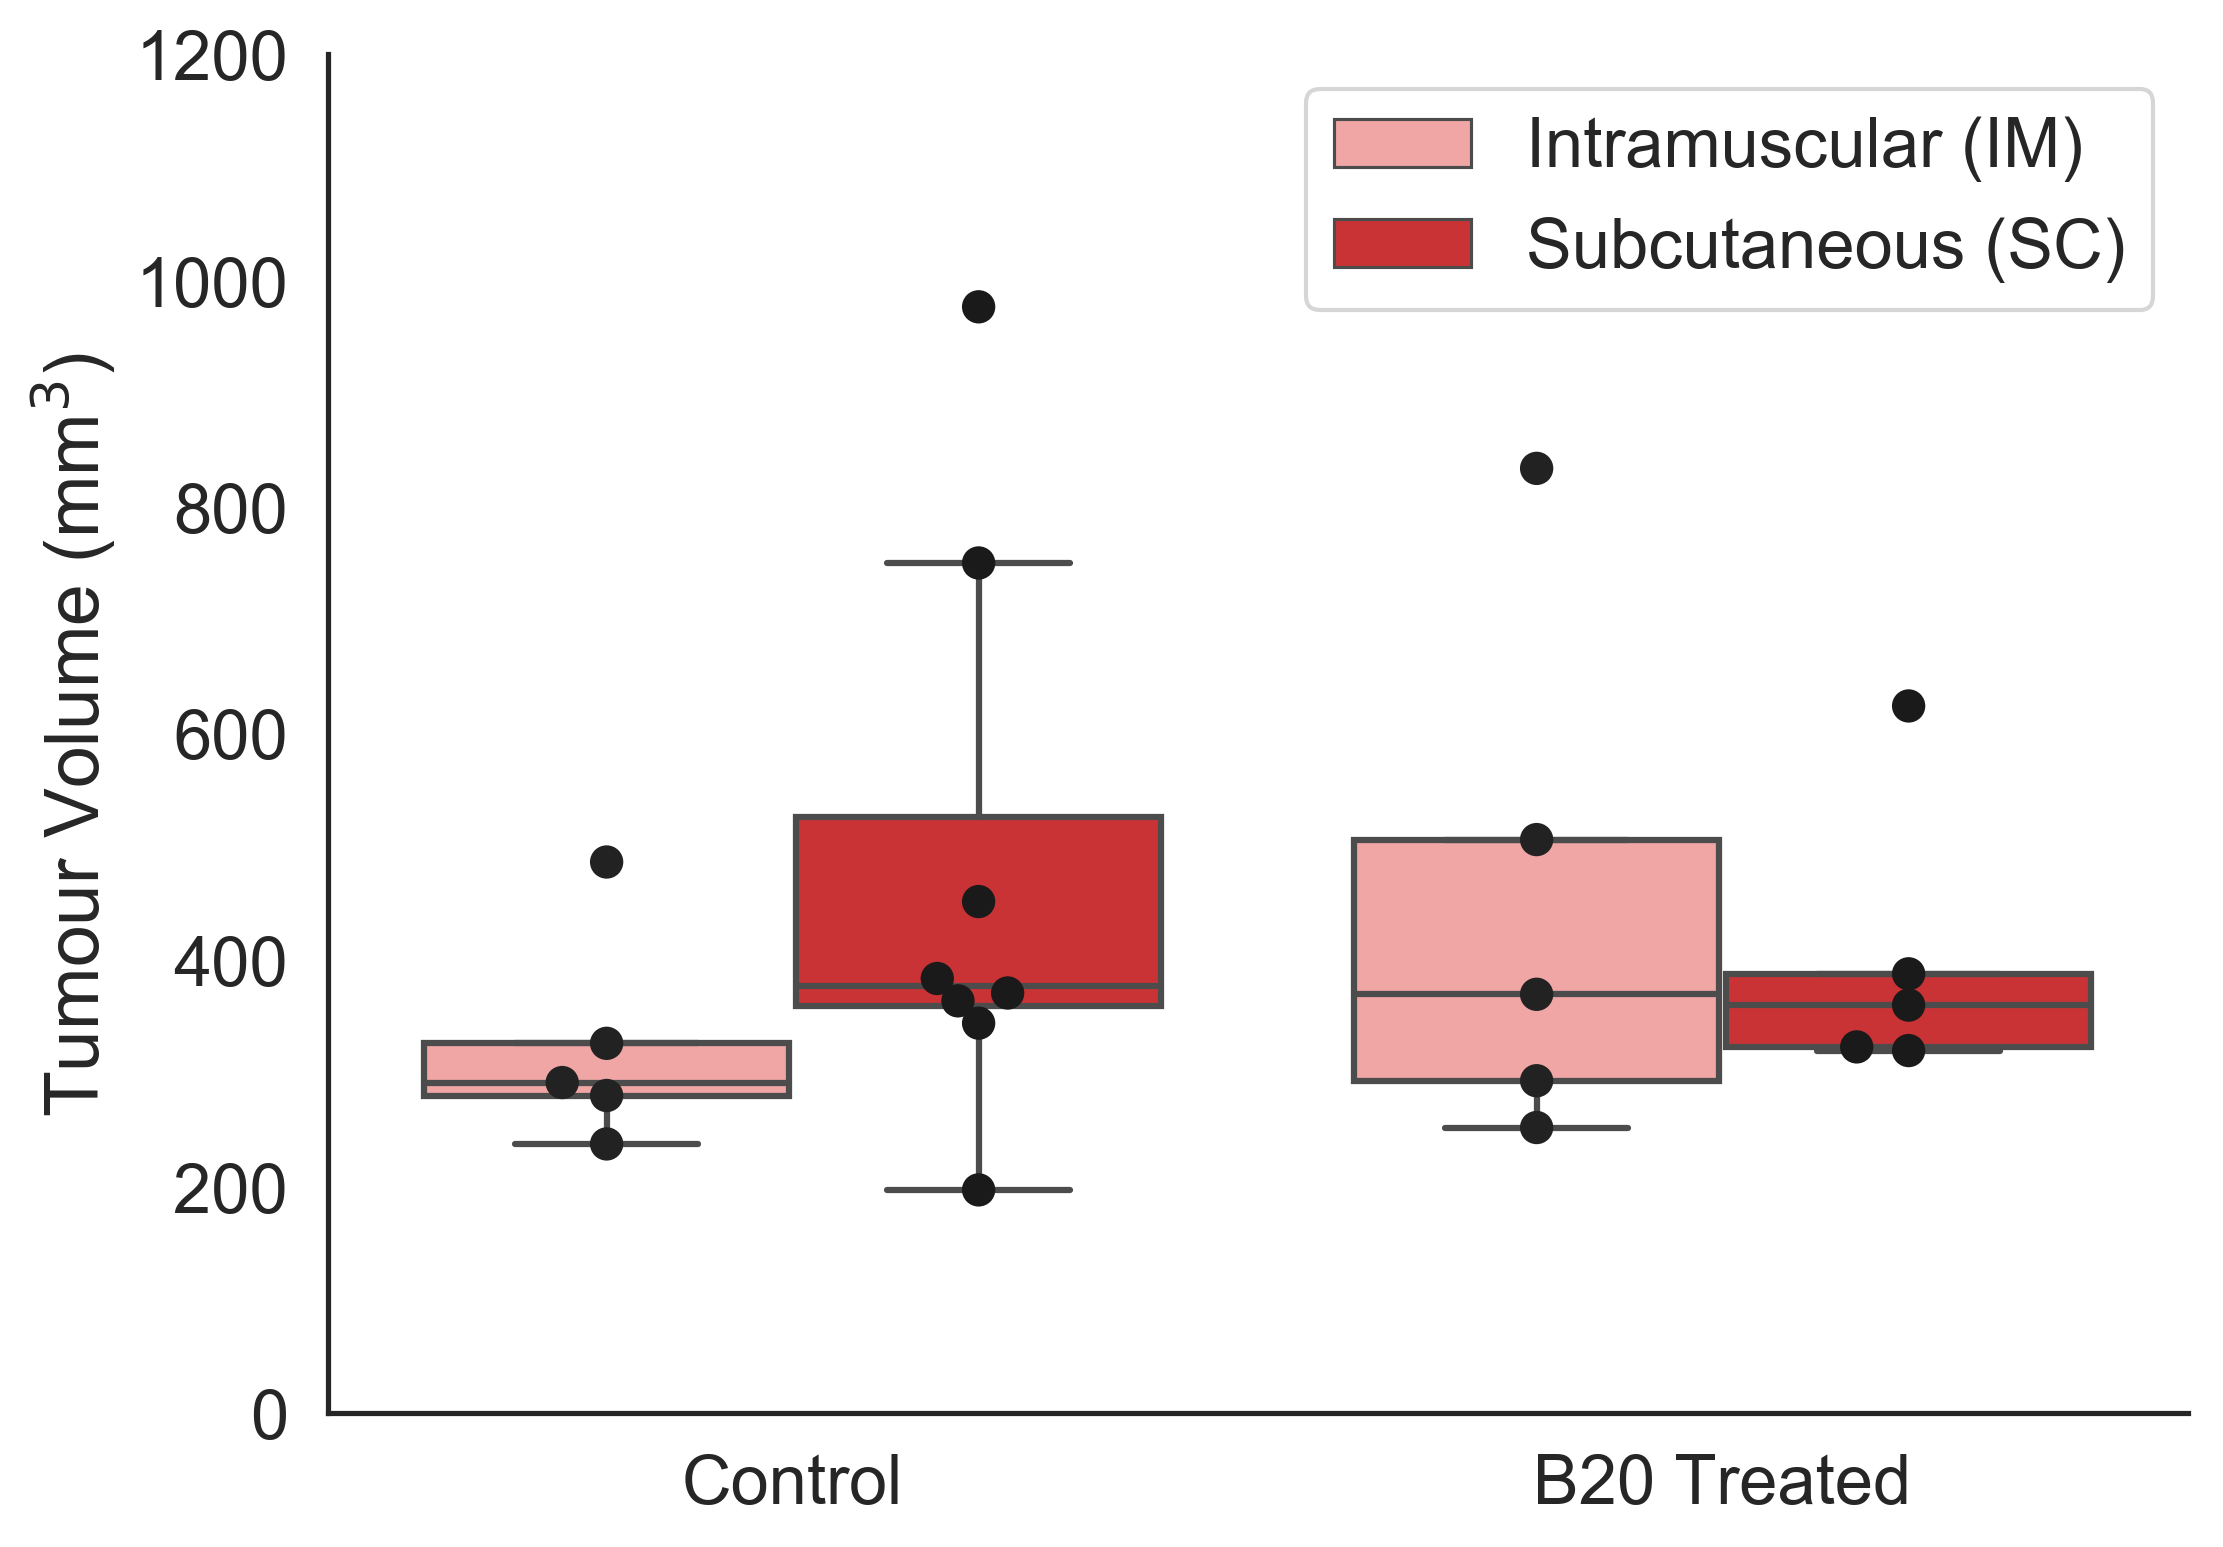
\includegraphics[width=\textwidth]{oemri_thesis3/oemri_thesis3-images/6_oep8_tumourVolumes.png} % requires the graphicx package
   \caption{Calculated tumour volumes from each of the four groups is shown. There were no statistically significant differences in tumour volumes amongst any of the groups.}
   \label{tumourVolumes}
\end{figure}

%\begin{figure}[htbp]
%   \centering
%   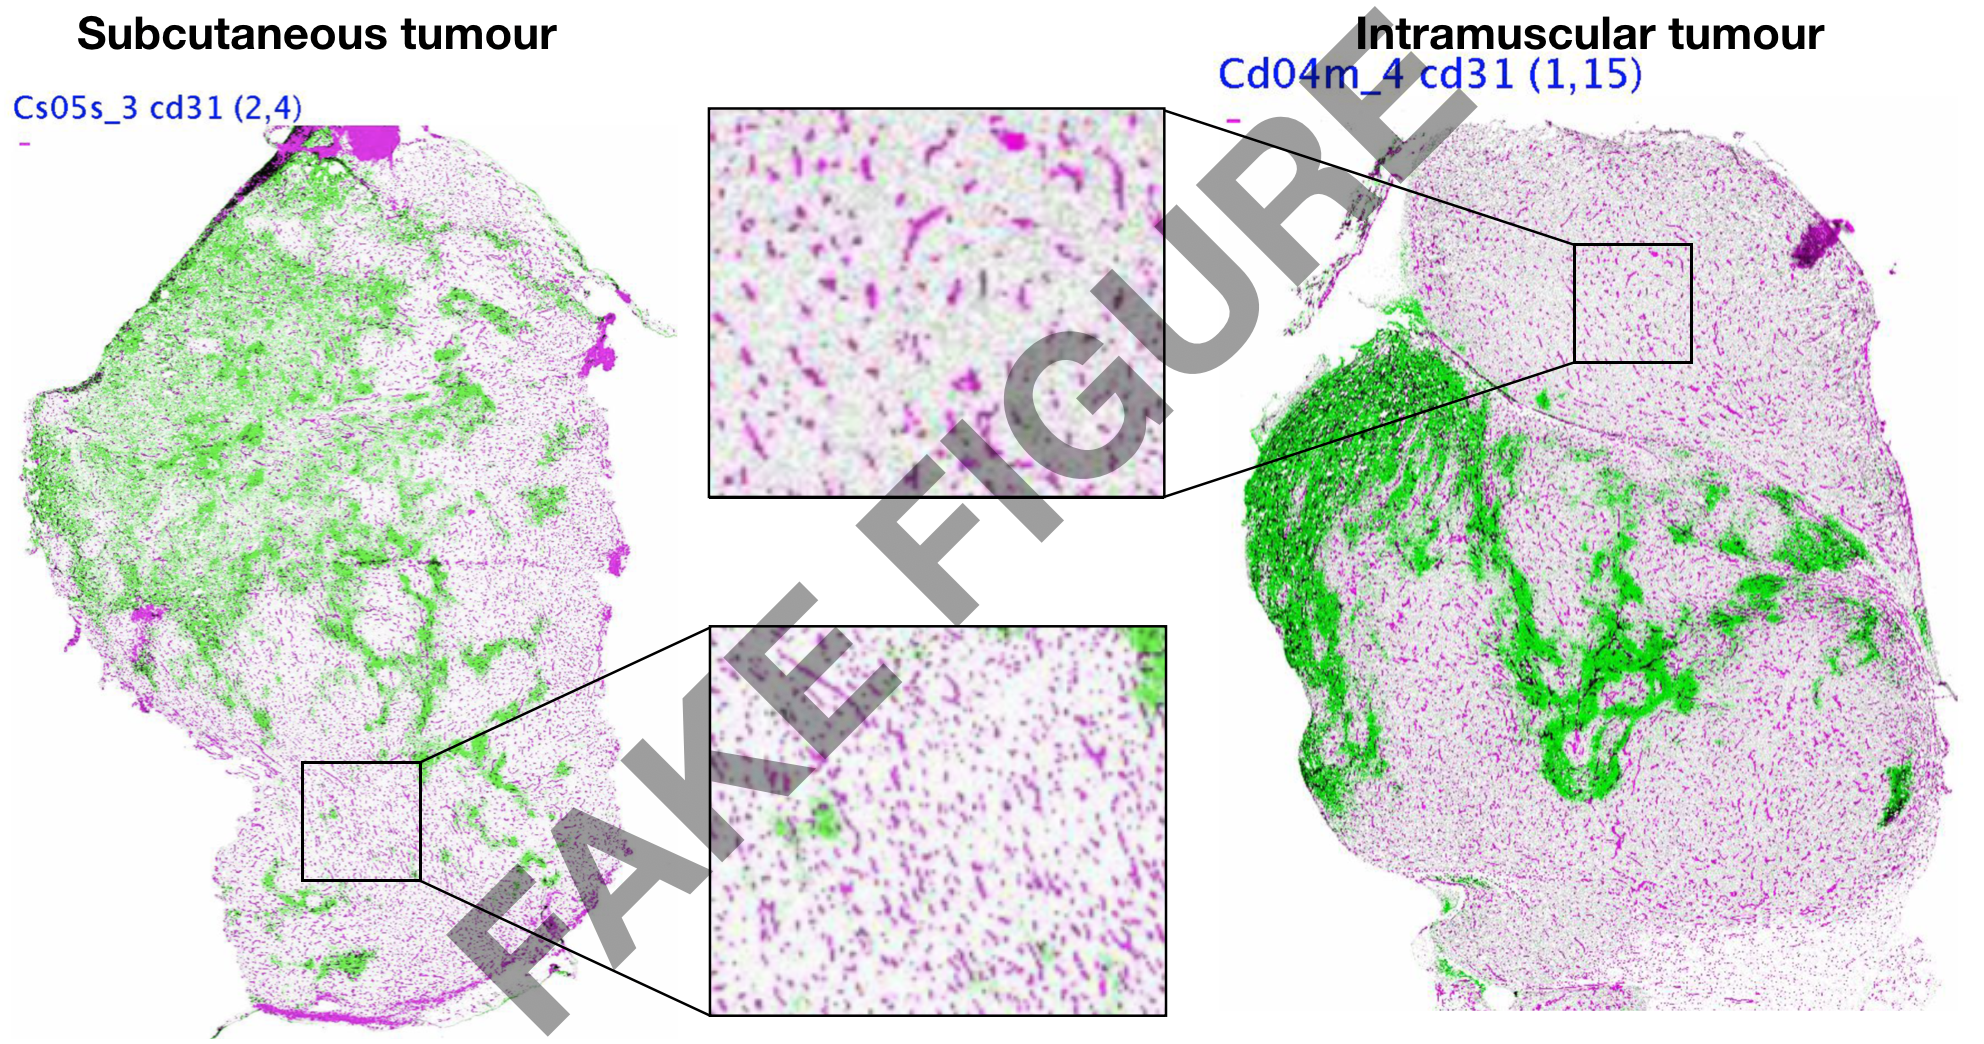
\includegraphics[width=\textwidth]{oemri_thesis3/oemri_thesis3-images/3_imsc_zoomed.png} % requires the graphicx package
%   \caption{example caption}
%   \label{imsc}
%\end{figure}

\subsection{Effects of B20 are dependent on the tumour microenvironment and baseline oxygenation}

To investigate whether the effects of antiangiogenic agents are dependent on different tumour microenvironments, mice were implanted with both \acs{IM} and \acs{SC} tumours. 
Tumours in this experiment were treated 24 hours prior to imaging.
To ensure the \acs{SC} tumours from mice with a double implant were similar to mice with only a single implant, three mice were implanted only with subcutaneous tumours.
No differences were found (data not shown), so the \acs{SC} tumours from this experiment were pooled together.

When comparing between \acs{SC} baseline and treated groups, there was a statistically significant difference (Mann-Whitney $U = 3.0, p = 0.007$) observed in mean \acs{NCWF} values for control (0.073 $\pm$0.009) vs. B20-treated tumours (0.119 $\pm$0.013) with a large effect size: Hedge's ${g=1.77}$ (Fig.~\ref{OEP8boxplot}).
However, no measurable difference in oxygenation was observed for the \acs{IM} tumours after B20 treatment (Mann-Whitney $U = 11.0, p = 0.42$).
Mean \acs{NCWF} from B20-treated \acs{IM} tumours was 0.137$\pm$0.018, and control \acs{IM} tumours was 0.146$\pm$0.017. 
Histological images (Fig.~\ref{allHisto}) also suggests that control \acs{IM} tumours have significantly less pimonidazole staining compared to \acs{SC} controls.
Furthermore, reduction in pimonidazole staining between control and treated \acs{IM} tumours is much lower compared to \acs{SC} tumours.
This provides clear evidence that the effects of B20 are dependent on the tumour microenvironment, and \acs{dOE-MRI} is sensitive to these differences.

\begin{figure}[htbp]
   \centering
   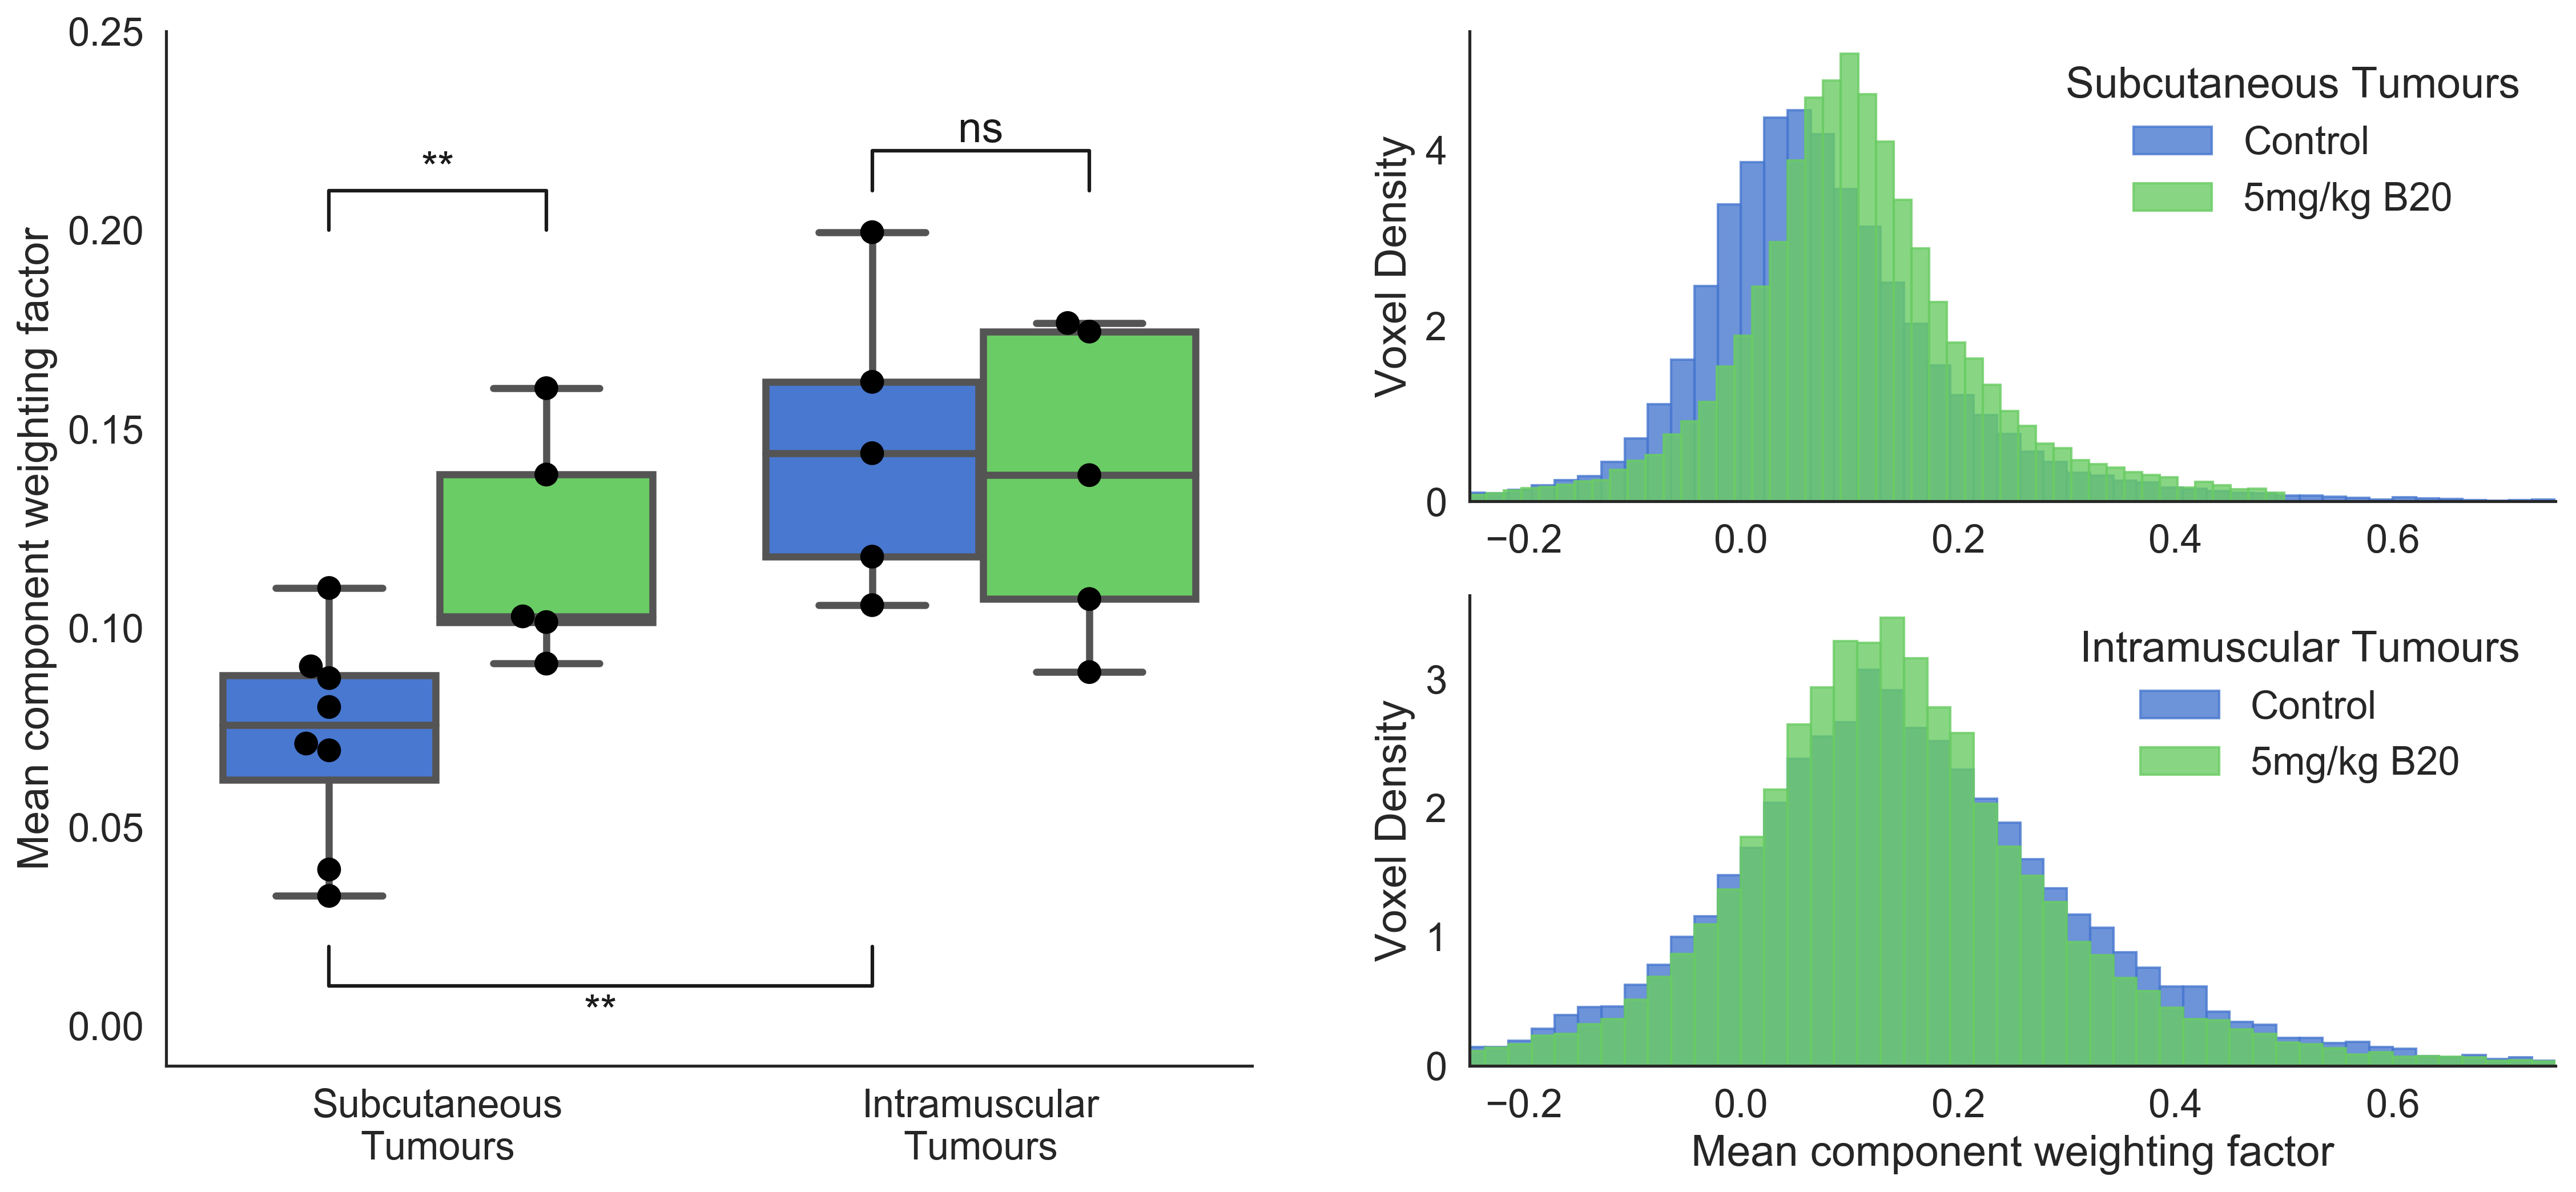
\includegraphics[width=\textwidth]{oemri_thesis3/oemri_thesis3-images/4_oep8_IMSC_b20_sanitized_dOEMRI.png} % requires the graphicx package
   \caption{\textbf{A)} Boxplot with four groups, 5mg/kg B20 treated and control mice with both \acs{SC} and \acs{IM} tumours.
   Differences between control \acs{SC} and \acs{IM} tumours, as well as control \acs{SC} and treated \acs{SC} tumours are statistically significant (Mann-Whitney U test; p $<$0.005, marked as **).
   There was no significantly difference in treated and control \acs{IM} tumours.
   \textbf{B)} Voxel density distributions of \acs{NCWF} for \acs{SC} (top) and \acs{IM} (bottom) treated and control tumours.
   Density distribution (i.e. normalized histograms) are shown rather than voxel counts due to uneven group size. 
   Note the shift of the \acs{IM} control tumours towards a higher \acs{NCWF} value.}
   \label{OEP8boxplot}
\end{figure}

\begin{figure}[htbp]
   \centering
   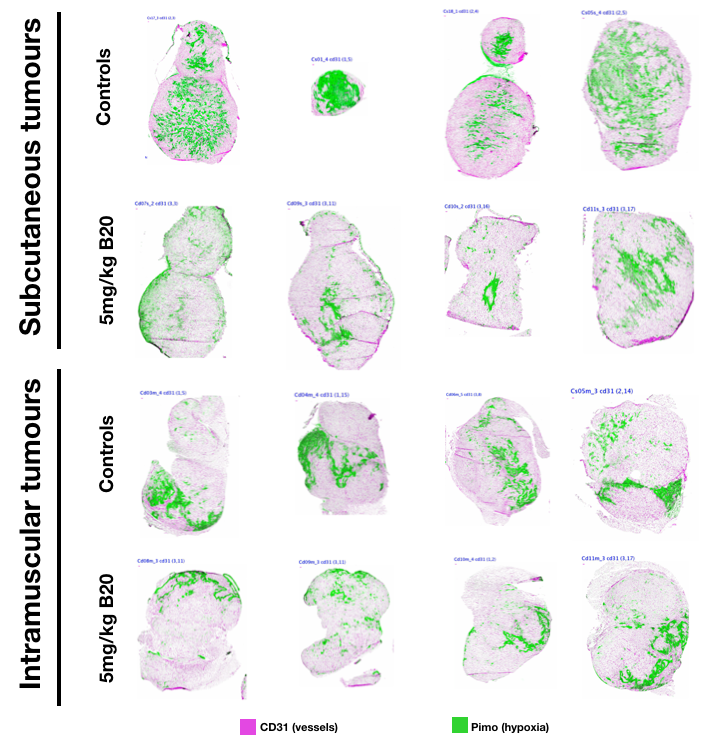
\includegraphics[width=\textwidth]{oemri_thesis3/oemri_thesis3-images/5_oep8_imsc_histo.pdf} % requires the graphicx package
   \caption{Representative histological sections from 16 total tumours of all four groups: 5mg/kg B20 treated and control mice with \acs{SC} and \acs{IM} tumours.
   Hypoxia marker pimonidazole staining is shown in green, and purple indicates the presence of blood vessels stained by CD31.}
   \label{allHisto}
\end{figure}

% ======================================================================
\section{Discussion}
% ======================================================================

% Bits and pieces from the latest grant pulled into this first paragraph
Hypoxic tumour cells may arise due to proliferation of cancer cells outpacing the growth of new vasculature, increasing the separation between blood vessels and forcing cells beyond the diffusion distance of oxygen from the blood supply. 
An alternative route to hypoxia is the consequence of poor flow, which can result in hypoxic tumour tissue due to depleted oxygen supply in the flowing blood or due to intermittent flow of poorly formed vessels. 
Tumour microenvironments are dynamic and highly heterogeneous, with variable vascular function and patterns of hypoxia.
However, the importance of hypoxia in tumours is well validated and undisputed; a meta-analysis of tumours from multiple origins found a consistent relationship between greater hypoxia in tumours and poorer outcomes with radiotherapy~\cite{Horsman:2012kw}.
While many techniques exist for measuring hypoxia in tumours, none have become clinical routine mainly owing to their expense, poor sensitivity and specificity, limited availability or their invasive nature~\cite{Colliez:2017fc,Baumann:2016gr}. 
For example, Eppendorf electrodes are sensitive and specific, and are a gold standard of measuring tissue hypoxia, but they are highly invasive, limited by sampling, and are not widely available. 
The accelerated radiotherapy, carbogen and nicotinamide (ARCON) trial demonstrated benefit in hypoxic tumours assessed retroactively using pimonidazole labeling of biopsy samples~\cite{Kaanders:2002wl}. 
However, immunohistochemical analyses of markers of hypoxia such as pimonidazole are invasive and do not sample the entire tumour.
A more widely applicable hypoxia-measuring tool that overcomes the availability, expense, invasiveness, sensitivity and specificity hurdles would be of high value for stratifying patients in hypoxia-targeted trials, prognostic imaging as well as for monitoring response to treatment. 

In this study we have demonstrated the utility of \acs{dOE-MRI} to assess tumour oxygenation changes after administration of B20.
Though this is not the first report of tumour oxygenation improvements after antiangiogenic drug treatment using MRI methods, we provide clear evidence this change is measurable using only the switching of inhaled gas and no injectable contrast agents.
Using electron paramagnetic resonance and an injectable paramagnetic tracer (triarylmethyl radical derivatives), Matsumoto et al.\ mapped increases in the partial pressure of oxygen in tumours after administration of the VEGF inhibiting antiangiogenic agent called sunitinib.
Two to four days following antiangiogenic treatment with sunitinib, they reported a transient improvement in oxygenation~\cite{Matsumoto:2011iv}.
Lemasson et al.\ obtained estimates of blood oxygen saturation using an ultrasmall super-paramagnetic iron oxide (\acs{USPIO}) contrast agent in a rat gliosarcoma model.
They reported that after sustained administration ($>$9 consecutive days) of the maximum dose of sorafenib, oxygen saturation in treated tumours reduced compared to untreated control tumours~\cite{Lemasson:2012dl}.
In this case, the dose and treatment schedule resulted in excessive pruning of the tumour vasculature to the point where drug and nutrient delivery became limited and tumour oxygenation actually reduced~\cite{Jain:2013jc}.
In our experiments, with the dose (5~mg/kg) and treatment schedule (single administration 24 or 48~h prior to imaging), we expected a vascular normalization effect corresponding to an increase in oxygenation~\cite{Chauhan:2012bm,Jain:2013jc,Huang:2012kn}.
Despite heterogeneity in amount and levels of oxygen response in the \acs{SC} tumours, we observed an overall increase in oxygenation after administering B20 (figures~\ref{dOEMRImaps},~\ref{aarts3boxplot}, and~\ref{OEP8boxplot}).

In this study we provided evidence that the location of tumour cell implants has a large impact on the microenvironment of the resulting solid tumour.
Tumour kinetics and responses to chemotherapies differ depending on the implant site and the effect of tumour implantation site is often not considered when assessing drug effect using \emph{in vivo} animal studies~\cite{Arjona:2006ch}.
Hubbard et al.\ compared the tumours derived from the VX2 rabbit carcinoma line implanted intramuscularly and intra-abdominally and discovered animals with \acs{IM} tumours had significantly higher levels of calcium compared to animals with intra-abdominal tumours~\cite{Hubbard:1980vf}.
This result was attributed to the differences in venous drainage of the two sites.
In another example, Malave et al.\ studied the Lewis-lung carcinoma model and reported a lower implant success rate for tumours implanted in the flank compared to the foot pad, and a higher rate of metastatic modules for tumours in the flank (indicating a reduced tumour-host immune response)~\cite{Malave:1979ui}.
Tumour implant site also alters growth kinetics and dramatically different tumour doubling times (in days) has been reported for implants in mouse tail (1.7), foot (1.6), chest (1.2), and leg (0.6)~\cite{Hill:1982ci}.
For the same amount of cells implanted, our experience is that \acs{IM} tumours typically grow much faster, have a more stable vascular architecture, less hypoxia (pimo staining), and increased vessel density (CD31 \%).
We attempted to control for this growth rate by injecting fewer cells for the \acs{IM} tumours. 
Our tumour volume measurements indicate there was no significant difference between the control \acs{IM} and \acs{SC} tumours despite the \acs{SC} tumours implanted with 5 times the amount of cells implanted.
We also showed that \acs{dOE-MRI} can assess increased baseline oxygenation in control tumours when the tumour site is changed from the dorsal subcutaneous region to the hind limb: \acs{IM} tumours have less pimonidazole staining compared to \acs{SC} tumours (figure~\ref{allHisto}).
%Figure~\ref{imsc} highlights some of these differences in representative SCCVII  tumours implanted \acs{SC} and \acs{IM}~\todo[backgroundcolor=red!20!white]{add some differences about tumours}.
Ultimately we showed that following treatment of \acs{IM} tumours with B20, no change in oxygenation was observed, likely because \acs{IM} tumours were already well-oxygenated.

To fully establish the utility of \acs{dOE-MRI} to assess tumour oxygenation non-invasively using inhaled oxygen or air, several subsequent experiments should be conducted.
Some ambiguities remain with a T$_1$-based \acs{dOE-MRI} method as its reflection of dissolved O$_2$ concentrations is complicated by complex, non-linear relationships with hemoglobin saturation and its effects on T$_2^*$, and with vascular perfusion and blood flow that may confound interpretation of existing \acs{dOE-MRI} signal.
These are further complicated by the array of physiological possibilities that may be visualized by a change in T$_1$. 
In future development of this method, the impact of T$_1$-weighting should be explored to ensure effects of interventions are not manifesting due to changes in tumour microenvironment that alter T$_1$.
An increase in T$_1$ suggests an oxygen-responsive area, while non-responding and negative-responding regions may represent a variety of physiologies. 
These areas may be completely unperfused and even necrotic, or they may be poorly perfused but viable, hypoxic tissues.
Further exploration of intermediate regions (i.e. not hypoxic or well-oxygenated) using \acs{dOE-MRI} and coupling it with \acs{BOLD}-MRI is warranted to fully classify all areas of the tumour. 
An unexplored application of \acs{dOE-MRI} is its potential to monitor treatment efficacy longitudinally as the contrast mechanism used is completely reversible. 
This opens up the possibility to do treatment interventions within a single imaging session with perfectly co-registered tumour volumes to allow for assessing oxygenation changes at the level of a single voxel.
Nevertheless, \acs{dOE-MRI} has tremendous potential for assessing tumour oxygenation as a non-invasive imaging method that is urgently needed in the clinic. 

% ======================================================================
\section{Conclusions}
% ======================================================================

Through this work we have shown that subcutaneously implanted SCCVII tumours treated with B20 and imaged 48h later are more oxygenated than control tumours. 
Additionally, we have established \acs{dOE-MRI} as a tool to assess baseline oxygenation level and demonstrated that \acs{IM} tumours are significantly more oxygenated than \acs{SC} tumours implanted in the same mice.
Finally we provided evidence that location of the tumour implant site has a large effect on therapy outcome as the more oxygenated \acs{IM} tumours did not respond to treatment with B20.
It is our expectation that after further refinement and expansion, this technique will become accessible and available in the clinic to screen cancer patients prior to chemo- or radiotherapy prescription, and be useful for developing new hypoxia-targeting drugs.




